\documentclass[11pt, oneside]{article}   	% use "amsart" instead of "article" for AMSLaTeX format
\usepackage{geometry}                		% See geometry.pdf to learn the layout options. There are lots.
\geometry{letterpaper}                   		% ... or a4paper or a5paper or ... 
%\geometry{landscape}                		% Activate for for rotated page geometry
%\usepackage[parfill]{parskip}    		% Activate to begin paragraphs with an empty line rather than an indent
\usepackage{graphicx}				% Use pdf, png, jpg, or eps§ with pdflatex; use eps in DVI mode
								% TeX will automatically convert eps --> pdf in pdflatex		
\usepackage{listings}
\usepackage{amssymb}
\usepackage{amsmath}
\usepackage{subfigure}

\lstset{language=Java, basicstyle=\scriptsize}


\title{CS675 Project 2: Get Started with RPC/RMI \\
Performance Evaluation of Game Server Protocols}
\author{Zhonghua Xi}
%\date{}							% Activate to display a given date or no date

\begin{document}
\maketitle

\section{Design}
\subsection{MMORPG}
The game is designed as a MMORPG (Massively multiplayer online role-playing game). Every user will control a role walking on a 2D tiled environment. Each tile can contain a treasure chest (with a random value associated with it) and multiple players. The first player on that tile who opens the chest will be awarded the treasure. After that the treasure will disappear. After all the chest were opened, the game is over, who gets the most score will win the game.

\subsubsection{Control}
Players use keyboard to control the movement of their roles in the virtual space and use space key to open a chest. They will be able to see where treasure boxes and other players are. Users will be notified other players' operations (movement, treasure boxes opened).

\subsection{GameWorld}
GameWorld class is the represantation of the current world, which also is the main game logic class which will be shared by all the servers and clients. GameWorld provides the following functionality: Generate random map, add/remove/update player, update Chest etc.

\subsection{Scene}
Scene class is the main UI class which will be shared by both RMI and Socket clients. Scene class relies on an object which implemented IClient interface to interact with the server, it contains a GameWorld object for rendering.

\section{Implementation}
\subsection{Server}
Once the server is started, it will generate a new map with treasure chests on the map with random locations and values.

\subsubsection{Socket Based Game Server}
One significant advantage of socket-based game server over RPC/RMI based server is that it can not only push update to each client, it can also broadcast the updates to all clients for certain events. (e.g., a new user entered the world, an existing user left the game)
While the later one can only pull information from server. Thus, besides the required two services (which is not used in socket-based server in practice), I also implemented the push version of the game server. Only changes (any player's location changed, chest opened, etc.) will be pushed to client, client will never call server to get the entire information of the world. This can significantly reduce network overhead (delay) thus improve user's experience.

\subsubsection{RMI Server}
Unlike socket-based server, RMI server doesn't know which client is calling, there is no session concept within. In order to distinguish different clients, each client will receive a unique token once they enter the game, and when they left the game, the token becomes invalid. During the game, most of the API calls must have the token as the first argument in order to distinguish clients.

\subsection{Client}
Once client is started, and connected to server. Then all the information of the world will be either pulled from client or pushed to client. These information will be used to render the world.
Fig.~\ref{fig:world} shows the world map from three different players' viewpoint.
The window title bar shows the current role's location, name and total score awarded.
Each green box in the world represents a treasure chest, each blue dot represents a player and the red dot represents the current player.
From Fig.~\ref{fig:world} we can see all the players were synced with the server.
\begin{figure*}[htbp] %  figure placement: here, top, bottom, or page
   \centering
   \subfigure[Player1]{\fbox{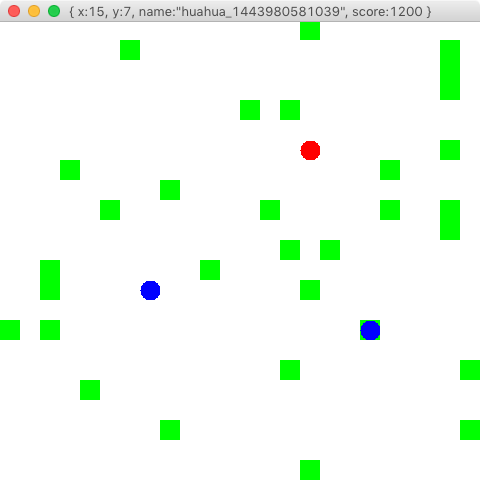
\includegraphics[width=2.8in]{figs/player1.png}}}
   \subfigure[Player2]{\fbox{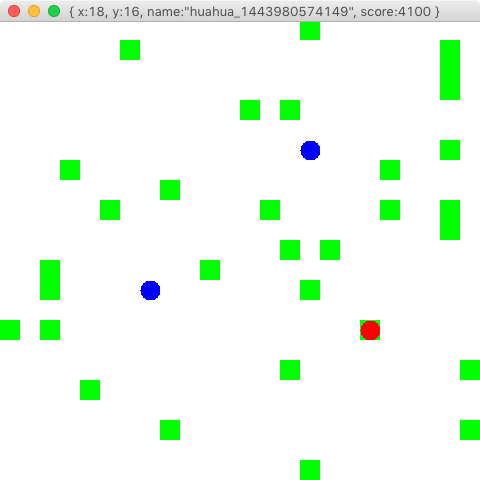
\includegraphics[width=2.8in]{figs/player2.png}}}
   \subfigure[Player3]{\fbox{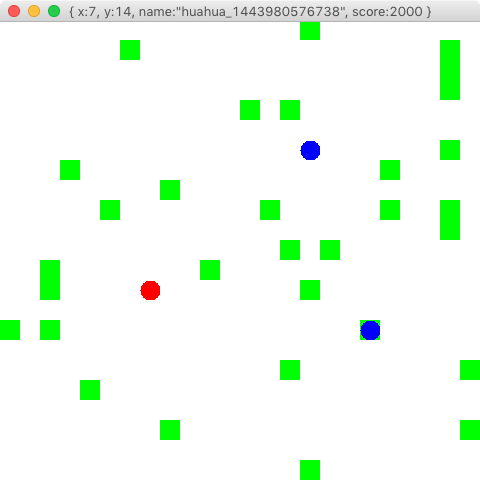
\includegraphics[width=2.8in]{figs/player3.png}}}
   \caption{World from different players' view.}
   \label{fig:world}
\end{figure*} 

\section{Performance Comparison}
\subsection{Methodology} 
Due to the difference in implementation of two type of game servers, it's hard to compare their performance directly based on the same functionality, such as openChest, two server will return different number of results to represent different update logic, total bytes transferred also differed from each other. In order to perform a fair comparison, I implemented echo method on both servers, which returns whatever client sent to the server.
The server runs on Medusa-node1, while the test client runs on Medusa-node2. 'System.nanoTime()' is used for high precision timing.

\subsection{Results}
I tested the average response time (over 1000 invocations) under different message sizes. 
From Fig~\ref{fig:response_time} we can see when message size is small ($<10kb$), socket-based server performs much better than RMI server, which is up to 75\% faster. However, when message size grows, the overhead (serialization, remote references, etc.) introduced by RMI becomes negligible, the bottleneck comes from the network.
\begin{figure*}[htbp] %  figure placement: here, top, bottom, or page
   \centering
   \includegraphics[width=5in]{figs/response_time.pdf}
   \caption{Response time for socket and RMI under different package size.}
   \label{fig:response_time}
\end{figure*} 

\subsection{Discussion}
Compare to socket-based server implementation, the performance of RMI server is somehow acceptable. However, as mentioned above, the main limitation is lack of pushing mechanism (bi-direction communication), which makes it inefficient as a game server (clients need to pull forever for not missing any updates of the world in a multi-player game). Although we can implement each client as a RMI server as well to enable the main game server invoking each client's method, it might not be possible in some cases.

\end{document}  